%==============================================================================
%  Internship Report — Modeling and Control of a PEM Fuel Cell Stack
%  Rules: see ../report_rules.md (UGA M1 EECS internship modalities)
%   - content (Introduction -> Conclusion) <= 25 pages
%     (title page, abstract, ToC, references, appendices excluded)
%   - no images in the main body: all figures live in Appendix B
%   - margins 1.5 cm on all sides
%  Build:  pdflatex main ; bibtex main ; pdflatex main ; pdflatex main
%==============================================================================
\documentclass[11pt,a4paper]{article}

% ----------------------------- Packages --------------------------------------
\usepackage[utf8]{inputenc}
\usepackage[T1]{fontenc}
\usepackage[english]{babel}
\usepackage[margin=1.5cm]{geometry}
\usepackage{amsmath,amssymb}
\usepackage{graphicx}
\graphicspath{{figures/}}
\usepackage{booktabs}
\usepackage{caption}
\usepackage{subcaption}
\usepackage{float}
\usepackage{enumitem}
\usepackage{chngcntr}
\usepackage{tikz}
\usetikzlibrary{arrows.meta,positioning,calc}
\usepackage[colorlinks=true,linkcolor=black,citecolor=blue,urlcolor=blue]{hyperref}

% ----------------------------- Title data ------------------------------------
\title{Modeling and Control of a PEM Fuel Cell Stack}
\author{Khalil Ellah \textsc{Lagha}}
\date{\today}

%==============================================================================
\begin{document}

% ----------------------------- 1. Title page ----------------------------------
\begin{titlepage}
\begin{center}
    \vspace*{1.5cm}
    {\scshape\LARGE Universit\'e Grenoble Alpes\par}
    {\large GIPSA-lab --- Infinity Team\par}
    \vspace{2.5cm}
    {\Large Internship Report\par}
    \vspace{0.6cm}
    \rule{\textwidth}{0.4pt}\\[0.5cm]
    {\huge\bfseries Modeling and Control of a PEM Fuel Cell Stack\par}
    \vspace{0.3cm}
    {\large From physical principles to per-cell calibration and dynamic characterization\par}
    \vspace{0.4cm}
    \rule{\textwidth}{0.4pt}
    \vspace{2.5cm}

    \begin{minipage}[t]{0.45\textwidth}
        \begin{flushleft}\large
        \emph{Author:}\\
        Khalil Ellah \textsc{Lagha}
        \end{flushleft}
    \end{minipage}
    \begin{minipage}[t]{0.45\textwidth}
        \begin{flushright}\large
        \emph{Supervisor:}\\
        Prof.\ Emmanuel \textsc{Witrant}
        \end{flushright}
    \end{minipage}

    \vfill
    {\large \today\par}
\end{center}
\end{titlepage}

% ----------------------------- 2. Abstract ------------------------------------
\begin{abstract}
\noindent
This report presents the modeling, calibration, and dynamic characterization of a
proton exchange membrane fuel cell (PEMFC) stack carried out at GIPSA-lab.
A reduced control-oriented model is developed from electrochemical principles:
a Nernst open-circuit voltage combined with semi-empirical activation, ohmic, and
concentration losses, coupled to lumped-volume hydrogen, membrane-hydration, and
cathode-humidity dynamics. Six parameters per cell are identified from the
Optimization Experiment using a two-stage optimization (differential evolution
followed by L-BFGS-B), yielding root-mean-square voltage errors below 12\,mV for
all healthy cells and revealing degraded cells through voltage collapse and
degenerate fits. The state-space matrices of the linearized model are written out
explicitly --- the state and input matrices follow directly from the dynamic
equations, while the output matrices require a Jacobian linearization of the
nonlinear voltage equation. The system is shown to be structurally controllable
for all realistic electro-osmotic drag coefficients, while a voltage-only output
observes the hydrogen pressure but not the water states. Step-load experiments
(3.3\,$\Omega$ and 6.8\,$\Omega$) characterize the current response of the stack
($\tau_I \approx 8$--$10$\,s), providing quantitative targets for closed-loop
control design. Building on these results, a control architecture based on a
DC/DC boost converter regulated by a PI controller is presented, in which the
converter output is regulated to behave either as a current source --- the
approach of Derbeli et al.\ --- or as a voltage source. All figures and detailed
tables are gathered in the appendices.
\end{abstract}

% ----------------------------- 3. Table of contents ---------------------------
\tableofcontents
\newpage

% ==============================================================================
\section{Introduction}
\label{sec:introduction}

Fuel cells convert the chemical energy of hydrogen directly into electricity, with
water and heat as the only by-products. Among them, the proton exchange membrane
fuel cell (PEMFC) is the leading candidate for transport and small stationary
applications thanks to its low operating temperature, high power density, and fast
start-up \cite{pukrushpan2003,daud2017pem}. Their efficient and safe operation,
however, requires feedback control of the gas supply and load: insufficient
reactant flow causes starvation and irreversible degradation, while excessive
anode--cathode pressure difference can damage the membrane \cite{zhu2017,kharrat2025}.
Control design, in turn, requires a model that is simple enough for analysis and
accurate enough to represent the actual hardware --- including the differences
between individual cells of a stack \cite{manana2006}.

This internship, carried out at GIPSA-lab (Universit\'e Grenoble Alpes) under the
supervision of Prof.~Emmanuel Witrant, addresses this need for a small educational
PEMFC stack of ten cells. The objectives are:
\begin{enumerate}[itemsep=1pt]
    \item to develop a reduced, control-oriented dynamic model of a single cell and
          of the stack, grounded in the electrochemical literature;
    \item to identify the model parameters \emph{per cell} from experimental data
          acquired on the bench;
    \item to derive the linearized state-space representation and analyze its
          structural controllability and observability, as a foundation for
          controller and observer design;
    \item to characterize experimentally the dynamic response of the stack to
          resistive load steps, providing the timescales needed for control
          bandwidth selection;
    \item to propose a PI-based control architecture for the PEMFC power system
          through a DC/DC boost converter, following \cite{derbeli2017}.
\end{enumerate}

The report is organized following a global vision of the work. Section~\ref{sec:context}
summarizes the operating principle of PEMFCs and positions the work in the
literature. Section~\ref{sec:methodology} presents the reduced model, the parameter
identification procedure, the state-space analysis method, and the experimental
protocols. Section~\ref{sec:results} discusses the calibration, structural-analysis,
and step-response results. Section~\ref{sec:control} presents the control of the
PEMFC power system with a DC/DC boost converter and a PI controller.
Section~\ref{sec:conclusion} concludes and outlines perspectives. In accordance with the report rules, all figures are gathered in
Appendix~\ref{app:figures} and detailed derivations and tables in
Appendices~\ref{app:ocv} and~\ref{app:tables}; the main text is self-contained and
readable without them.

% ==============================================================================
\section{Context \& Background}
\label{sec:context}

\subsection{Operating principle of a PEM fuel cell}

A PEMFC converts the chemical energy of hydrogen and oxygen into electricity,
heat, and water \cite{manana2006,mohiuddin2018,thomya2011}. At the anode, hydrogen
splits into protons and electrons; the protons cross the polymer membrane while the
electrons supply the external load; at the cathode, oxygen recombines with both to
form water (see Appendix~\ref{app:figures}, Figure~\ref{fig:pemfc-operation}). The
overall reaction is
\begin{equation*}
    \mathrm{H_2 + \tfrac{1}{2}O_2 \rightarrow H_2O + electricity + heat}.
\end{equation*}
The membrane conducts protons, blocks electrons, and separates fuel from oxidant;
together with the two electrodes it forms the membrane electrode assembly (MEA)
\cite{manana2006,ionescu2020}. Water management is critical: a dry membrane loses
proton conductivity, while excess water floods the gas paths; stable operation
requires a balance between the two \cite{weber2004,zhang2017}.

\subsection{Voltage losses and polarization behavior}

A practical cell delivers less than the reversible voltage because of three loss
mechanisms \cite{manana2006,pukrushpan2003,thanapalan2008}, dominant in different
regions of the polarization curve (Appendix~\ref{app:figures},
Figure~\ref{fig:pemfc-losses}):
\begin{itemize}[itemsep=1pt]
    \item \textbf{activation loss} --- kinetic limitation of the electrode
          reactions, dominant at low current \cite{pukrushpan2003,weber2004};
    \item \textbf{ohmic loss} --- resistive drop across membrane and conductors,
          approximately linear in current \cite{pukrushpan2003,thanapalan2008};
    \item \textbf{concentration loss} --- mass-transport limitation causing the
          sharp voltage drop at high current density \cite{manana2006,weber2004}.
\end{itemize}
The fast transient behavior is additionally shaped by the charge double-layer
effect at the electrode/electrolyte interface, which acts as a small capacitor in
equivalent electrical models \cite{pukrushpan2003,manana2006}.

\subsection{State of the art}

Control-oriented PEMFC modeling traces back to the system-level model of
Pukrushpan \cite{pukrushpan2003}, which combines a polarization-curve voltage model
with compressor, manifold-filling, and membrane-hydration dynamics, and which most
later models specialize or simplify \cite{thanapalan2008,kim2010,zhu2017}.
Simplified electrical models reproduce the static $V$--$I$ characteristic of small
stacks with a handful of parameters \cite{manana2006,shen2005}; importantly,
per-cell measurements on a small stack show voltage deviations of up to 7\,\%
between cells \cite{manana2006}, motivating the per-cell calibration adopted here.
Parameter identification by direct-search optimization on measured voltage and
power was formalized in \cite{thanapalan2008}, and modern metaheuristics extend it
\cite{cao2019}. On the control side, PI regulation of flows, pressures, and
converter currents is the established baseline \cite{zhu2017,derbeli2017},
with LQ multivariable control, time-delay control, and predictive schemes as
documented upgrades \cite{pukrushpan2003,kim2010,wang2021simulation}. At system
level, the delays of the air and hydrogen supply components remain the limiting
factor for dynamic operation \cite{kharrat2025}. A thematic synthesis of these
references is maintained in the project documentation.

% ==============================================================================
\section{Methodology}
\label{sec:methodology}

\subsection{Reduced control-oriented model}
\label{sec:model}

Following \cite{thanapalan2008,pukrushpan2003}, the cell is decomposed into three
interacting parts --- anode, membrane, and cathode --- each lumped into a single
control volume. The main assumptions are: hydrogen and air are the only reactants;
channel pressure drops are neglected; gases follow the ideal-gas law; temperature
is constant or slowly varying; and the oxygen partial pressure is fixed at
$P_{O_2}^{\ast}=0.21\,P_{\mathrm{atm}}$. The result is a semi-empirical reduced
model: physically motivated mass balances combined with empirical loss relations
that are calibrated from data \cite{cao2019}.

\paragraph{Open-circuit voltage.}
The reversible voltage follows from the Gibbs free energy of the reaction and
Faraday's law (full derivation in Appendix~\ref{app:ocv}):
\begin{equation}
    \label{eq:ocv}
    E = 1.229 - 0.85\times10^{-3}(T_{fc}-298.15)
      + 4.31\times10^{-5}\,T_{fc}\left[\ln p_{H_2} + \tfrac{1}{2}\ln p_{O_2}\right]\;\mathrm{V},
\end{equation}
with $T_{fc}$ the stack temperature [K] and $p_{H_2}$, $p_{O_2}$ the reactant
partial pressures [atm] \cite{pukrushpan2003}.

\paragraph{Voltage losses.}
The cell voltage is the reversible voltage minus three losses:
\begin{equation}
    \label{eq:vfc}
    v_{fc} = E - v_{act} - v_{ohm} - v_{con},
\end{equation}
with the semi-empirical forms \cite{pukrushpan2003,thanapalan2008,cao2019}
\begin{align}
    v_{act} &= \xi_1+\xi_2 T+\xi_3 T\ln(C_{O_2})+\xi_4 T\ln(i_{FC}),
    \label{eq:vact}\\
    v_{ohm} &= i_{FC}\Bigl(\rho_m\frac{t_m}{A_{fc}}+c\Bigr),
    \qquad
    \rho_m = \Bigl[(b_{11}\lambda_m-b_{12})
              \exp\bigl(b_2(\tfrac{1}{303}-\tfrac{1}{T_{fc}})\bigr)\Bigr]^{-1},
    \label{eq:vohm}\\
    v_{con} &= -B\ln\Bigl(1-\frac{i_{FC}}{i_{\max}}\Bigr),
    \label{eq:vcon}
\end{align}
where $i_{FC}$ is the cell current, $C_{O_2}$ the dissolved-oxygen concentration
(Henry's law), $t_m$ and $A_{fc}$ the membrane thickness and active area,
$\lambda_m$ the membrane water content, and
$\boldsymbol{\theta}=(\xi_1,\xi_2,\xi_3,\xi_4,B,c)$ the parameters identified per
cell. The stack voltage is the sum over the $n$ cells in series.

\paragraph{Anode dynamics.}
The hydrogen pressure follows a mass balance on the anode volume with Faraday
consumption:
\begin{equation}
    \label{eq:anode}
    \dot{P}_{H_2}=\frac{R_{H_2}T}{V_{an}}
    \Bigl(W_{H_2,in}-W_{H_2,out}-\frac{M_{H_2}n}{2F}\,i_{FC}\Bigr),
\end{equation}
and the anode water balance retains only the membrane flux,
$\dot{m}_{w,an}=W_{v,mbr}$, with relative humidity
$\phi_{an}=m_{w,an}R_vT/(V_{an}p_{sat}(T))$. $P_{H_2}$ enters the Nernst term of
\eqref{eq:ocv} and is the primary control target.

\paragraph{Membrane and cathode.}
Water crosses the membrane mainly by electro-osmotic drag,
$W_{v,mbr}=M_v A_{fc}\,n\,n_d\,i_{FC}/F$ \cite{pukrushpan2003}; the membrane water
content is given by the Springer sorption isotherm
$\lambda(a)=0.043+17.81a-39.85a^2+36.0a^3$ averaged over the two faces. On the
cathode side, the oxygen partial pressure is held constant at
$P_{O_2}^{\ast}=0.21\,P_{\mathrm{atm}}$, which removes the oxygen state while
keeping the cathode water balance,
$\dot{m}_{w,ca}=-W_{v,mbr}+W_{v,gen}$ with $W_{v,gen}=M_v n\,i_{FC}/(2F)$,
whose humidity feeds back into the ohmic loss through $\lambda_m$. The
block-level architecture of the resulting model is shown in
Appendix~\ref{app:figures}, Figure~\ref{fig:architecture}. The model is compact
and suitable for simulation and control design, at the price of ignoring spatial
variations, oxygen transients, and detailed liquid-water effects
\cite{weber2004,zhang2017}.

\subsection{Per-cell parameter identification}
\label{sec:identification}

The six parameters per cell are identified by minimizing the root-mean-square
error (RMSE) between predicted and measured cell voltage over a calibration window:
\begin{equation}
    \min_{\boldsymbol{\theta}}\;
    \sqrt{\frac{1}{N}\sum_{i=1}^{N}
        \bigl(v_{\text{model}}(I_i,P_{H_2,i};\boldsymbol{\theta})-v_{\text{meas},i}\bigr)^2}.
    \label{eq:rmse}
\end{equation}
A two-stage strategy is used: \textbf{differential evolution} for the global
search (population 20, up to 800 generations, fixed seed), followed by
\textbf{L-BFGS-B} local refinement under the same box bounds. Physical constraints
are imposed as bounds: $\xi_4\le 0$, $B\ge 0$, $c\ge 0$. The optimizer converges
for most cells within a few tens of generations (convergence history in
Appendix~\ref{app:figures}, Figure~\ref{fig:cost-evolution}).

\subsection{State-space analysis}
\label{sec:ss-method}

Around an operating point $(\mathbf{x}_0,\mathbf{u}_0)$ the model is put in the
standard linear state-space form
$\dot{\mathbf{x}}=A\mathbf{x}+B\mathbf{u}$, $y=C\mathbf{x}+D\mathbf{u}$.
Controllability is assessed through the rank of
$\mathcal{C}=[B\;AB\;A^2B]$ and observability through
$\mathcal{O}=[C;\,CA;\,CA^2]$. The explicit construction of the four matrices ---
$A$ and $B$ read off the dynamic equations, $C$ and $D$ obtained by Jacobian
linearization of the nonlinear voltage equation --- is carried out in
Section~\ref{sec:ctrb-obsv}.

\subsection{Experimental protocols}
\label{sec:protocols}

All experiments were performed on the ten-cell educational PEMFC stack of the
laboratory bench, with per-cell voltage acquisition at 1\,Hz through the serial
data-acquisition chain developed in the project.
\begin{itemize}[itemsep=1pt]
    \item \textbf{Optimization Experiment} (April 2026): a fixed $25\,\Omega$
          resistor is connected at $t=135$\,s and removed at $t=684$\,s, with no
          valve-driven current control. The calibration points used for the
          per-cell parameter identification are drawn from the loaded window of
          this experiment.
    \item \textbf{TR-current step experiments} (9 June 2026): the stack is left at
          open circuit, then a fixed resistor ($3.3\,\Omega$ for Experiment~1,
          $6.8\,\Omega$ for Experiment~4) is connected at $t=0$. The processing
          pipeline detects the connection event from a $>100$\,mA current jump and
          re-zeros the time axis. The current step response is fitted with the
          exponential model
          $I(t)=I_{\text{ss}}+\Delta I\,e^{-t/\tau_I}$, from which settling times
          $T_{s,p\%}=-\tau_I\ln(p/100)$ are derived analytically; the
          90\,\%$\to$10\,\% fall time is measured on the raw signal.
\end{itemize}

% ==============================================================================
\section{Results \& Analysis}
\label{sec:results}

\subsection{Parameter identification on the Optimization Experiment}
\label{sec:results-identification}

The two-stage optimizer identified the six semi-empirical parameters for all ten
cells from the loaded window of the Optimization Experiment. For the healthy cells
the calibration RMSE ranges from 2.0 to 11.3\,mV --- below 12\,mV in all cases ---
and the mean time-series RMSE over the healthy cells is 8.0\,mV. The per-cell
$V$--$I$ fits, the time-series comparison, the stack-level validation, and the
error traces are shown in Appendix~\ref{app:figures},
Figures~\ref{fig:vi-opt}--\ref{fig:ts-opt-error}; the complete table of tuned
parameters is given in Appendix~\ref{app:tables}, Table~\ref{tab:params-opt}.

Two findings stand out. First, the model describes healthy cells accurately with
only six parameters: the identified activation coefficients are consistent across
cells, and the concentration ($B$) and contact-resistance ($c$) terms remain
small, indicating that activation and ohmic effects dominate over the covered
operating range. Second, the identification doubles as a \emph{diagnosis} tool:
Cells~0, 1, and~2 collapse to approximately 0\,V under load and the optimizer
returns identical, degenerate parameter sets for them (RMSE $<0.1$\,mV against a
flat near-zero voltage) --- a clear signature of hardware degradation rather than
a physically meaningful fit, since no consistent parameter combination within the
physical bounds can reproduce a non-functioning electrode.

\subsection{State-space representation, controllability and observability}
\label{sec:ctrb-obsv}

\subsubsection{State-space representation of the fuel cell}

The linearized model uses the state, input, and output vectors
\begin{equation*}
    \mathbf{x} = \begin{bmatrix} P_{H_2} \\ m_{w,an} \\ m_{w,ca} \end{bmatrix},
    \qquad
    \mathbf{u} = \begin{bmatrix} i_{FC} \\ W_{H_2,in} \end{bmatrix},
    \qquad
    y = v_{fc},
\end{equation*}
where $P_{H_2}$ is the anode hydrogen partial pressure, $m_{w,an}$ and $m_{w,ca}$
the water masses stored on the anode and cathode sides, $i_{FC}$ the load current
(a disturbance imposed by the load), $W_{H_2,in}$ the hydrogen inlet flow (the
manipulated input), and $v_{fc}$ the measured cell voltage. In the standard form
$\dot{\mathbf{x}}=A\mathbf{x}+B\mathbf{u}$, $y=C\mathbf{x}+D\mathbf{u}$, the four
matrices have a direct physical reading: $A$ describes the internal dynamics
(water exchange across the membrane; the hydrogen pressure behaves as an
integrator), $B$ describes how the current drawn and the inlet flow drive the
states, $C$ describes how the states appear in the measured voltage, and $D$ is
the direct feedthrough from the inputs to the voltage.

\paragraph{Matrices $A$ and $B$ --- read directly from the dynamic equations.}
The three state equations of Section~\ref{sec:model} are linear in the states and
inputs once the temperature is held constant: the hydrogen pressure balance
\eqref{eq:anode} (with $W_{H_2,out}\approx 0$ for the dead-end anode) and the two
water balances written on the membrane water-transport terms,
\begin{equation*}
    \dot{m}_{w,an} = -\beta\, m_{w,an} + \gamma\, m_{w,ca} + d_1\, i_{FC},
    \qquad
    \dot{m}_{w,ca} = \beta\, m_{w,an} - \gamma\, m_{w,ca} + d_2\, i_{FC},
\end{equation*}
with
$\beta = D_w/(V_{an}t_m)$, $\gamma = D_w/(V_{ca}t_m)$,
$d_1 = n_d M_v/F$, and $d_2 = (n-2n_d)M_v/(2F)$.
No linearization is needed; the matrices follow immediately:
\begin{equation}
    A =
    \begin{bmatrix}
        0 & 0 & 0\\[2pt]
        0 & -\beta & \gamma\\[2pt]
        0 & \beta & -\gamma
    \end{bmatrix},
    \qquad
    B =
    \begin{bmatrix}
        -\dfrac{R_{H_2}T\,M_{H_2}\,n}{2F\,V_{an}} & \dfrac{R_{H_2}T}{V_{an}}\\[8pt]
        d_1 & 0\\[2pt]
        d_2 & 0
    \end{bmatrix}.
    \label{eq:AB}
\end{equation}
The first column of $B$ is the effect of the load current (hydrogen consumption
and electro-osmotic water displacement); the second column shows that the inlet
flow acts on the hydrogen pressure only.

\paragraph{Matrices $C$ and $D$ --- obtained by Jacobian linearization.}
Unlike the state equations, the output equation
$y = v_{fc} = E(P_{H_2}) - v_{act}(i_{FC}) - v_{ohm}(i_{FC},\lambda_m(m_{w,an},m_{w,ca})) - v_{con}(i_{FC})$
is \emph{nonlinear} in both states and inputs --- it contains logarithms of
$P_{H_2}$ and $i_{FC}$ and the nonlinear membrane-resistivity law
\eqref{eq:vohm} --- so $C$ and $D$ cannot be read off the equations. They are
obtained by a first-order Taylor (Jacobian) expansion around the operating point
$(\mathbf{x}_0,\mathbf{u}_0)$:
\begin{equation*}
    \delta y \;\approx\;
    \underbrace{\left.\frac{\partial v_{fc}}{\partial \mathbf{x}}\right|_{(\mathbf{x}_0,\mathbf{u}_0)}}_{C}\,
    \delta\mathbf{x}
    \;+\;
    \underbrace{\left.\frac{\partial v_{fc}}{\partial \mathbf{u}}\right|_{(\mathbf{x}_0,\mathbf{u}_0)}}_{D}\,
    \delta\mathbf{u}.
\end{equation*}
The three steps are:
\begin{enumerate}[itemsep=1pt]
    \item \emph{Hydrogen-pressure entry.} Only the Nernst term \eqref{eq:ocv}
          depends on $P_{H_2}$:
          $\partial v_{fc}/\partial P_{H_2}
           = 4.31\times10^{-5}\,T/P_{H_2,0}$.
    \item \emph{Water-state entries.} The water masses act on the voltage through
          the chain
          $m_{w}\rightarrow \phi \rightarrow \lambda_m \rightarrow \sigma_m
           \rightarrow v_{ohm}$. Differentiating this chain gives
          \begin{equation*}
              \frac{\partial v_{fc}}{\partial m_{w,an}}
              = \kappa_0\,\lambda'(\phi_{an,0})\,\frac{R_v T}{2V_{an}p_{sat}(T)},
              \qquad
              \frac{\partial v_{fc}}{\partial m_{w,ca}}
              = \kappa_0\,\lambda'(\phi_{ca,0})\,\frac{R_v T}{2V_{ca}p_{sat}(T)},
          \end{equation*}
          with
          $\kappa_0 = i_0 t_m b_{11}
           \exp\bigl[b_2(\tfrac{1}{303}-\tfrac{1}{T})\bigr]/(A_{fc}\,\sigma_{m,0}^{2})$
          and $\lambda'(a)=17.81-79.70a+108a^2$ (derivative of the Springer
          isotherm).
    \item \emph{Input entries.} Differentiating the three loss terms with respect
          to $i_{FC}$ at $i_0$, and noting that $W_{H_2,in}$ does not enter the
          output equation directly:
          \begin{equation*}
              \frac{\partial v_{fc}}{\partial i_{FC}}
              = -\Bigl(\frac{\xi_4 T}{i_0}
                + \rho_{m,0}\frac{t_m}{A_{fc}} + c
                + \frac{B}{i_{\max}-i_0}\Bigr),
              \qquad
              \frac{\partial v_{fc}}{\partial W_{H_2,in}} = 0.
          \end{equation*}
\end{enumerate}
The resulting output matrices at the operating point are
\begin{equation}
    C =
    \begin{bmatrix}
        \dfrac{4.31\times10^{-5}\,T}{P_{H_2,0}} &
        \kappa_0\,\lambda'(\phi_{an,0})\,\dfrac{R_v T}{2V_{an}p_{sat}(T)} &
        \kappa_0\,\lambda'(\phi_{ca,0})\,\dfrac{R_v T}{2V_{ca}p_{sat}(T)}
    \end{bmatrix},
    \label{eq:Cmat}
\end{equation}
\begin{equation}
    D =
    \begin{bmatrix}
        -\Bigl(\dfrac{\xi_4 T}{i_0}
        + \rho_{m,0}\dfrac{t_m}{A_{fc}} + c
        + \dfrac{B}{i_{\max}-i_0}\Bigr) & 0
    \end{bmatrix}.
    \label{eq:Dmat}
\end{equation}
In the \emph{simplified} model where $\lambda_m$ is held constant, the two
water-state entries of $C$ vanish and
$C_{\text{red}} = \bigl[\,4.31\times10^{-5}\,T/P_{H_2,0}\;\;0\;\;0\,\bigr]$.

\subsubsection{Controllability}

Because $P_{H_2}$ is directly driven by $W_{H_2,in}$ (entry
$R_{H_2}T/V_{an}>0$ in $B$), controllability of the full system reduces to
controllability of the two-state water subsystem
$(A_w,B_w)$ with
$A_w=\bigl[\begin{smallmatrix}-\beta & \gamma\\ \beta & -\gamma\end{smallmatrix}\bigr]$
and $B_w=[d_1;\,d_2]$ from \eqref{eq:AB}. Its controllability determinant,
$\det(\mathcal{C}_w)=(d_1+d_2)(\beta d_1-\gamma d_2)$ with
$d_1+d_2=nM_v/(2F)>0$, vanishes only under the single degenerate condition
\begin{equation}
    n_d = \frac{n\,V_{an}}{2\,(V_{an}+V_{ca})},
    \label{eq:ctrb-cond}
\end{equation}
i.e.\ when electro-osmotic drag exactly cancels the back-diffusion transport.
\textbf{The system is therefore fully controllable for all physically realistic
drag coefficients.}

\subsubsection{Observability}

With voltage as the only measurement, the observability matrix
$\mathcal{O}=[C;\,CA;\,CA^2]$ is built from \eqref{eq:Cmat}. In the simplified
model the output reduces to $C_{\text{red}}$:
\textbf{voltage observes the hydrogen pressure but not the two water states.}
In the full model all three states are potentially observable, but the
water-state sensitivities in \eqref{eq:Cmat} are small and degrade away from the
operating point. The practical consequence is that hydrogen-pressure regulation
can rely on a reduced-order voltage-based observer, whereas a full-state observer
would require additional pressure or humidity sensors.

\subsection{Step-response characterization (TR-current experiments)}
\label{sec:results-tr}

In both step experiments, Cells~1 and~2 read approximately 0\,mV throughout the
loaded window, confirming the degradation first observed in the Optimization
Experiment; all other cells behave normally. The measured channels and the
annotated step responses are shown in Appendix~\ref{app:figures},
Figures~\ref{fig:tr-experiments} and~\ref{fig:tr-responses}.
Table~\ref{tab:response-rt} summarizes the metrics.

\begin{table}[H]
    \centering
    \caption{Response-time metrics for the current step response.}
    \label{tab:response-rt}
    \small
    \begin{tabular}{lcc}
        \toprule
        \textbf{Current metric} & \textbf{Exp~1 (3.3\,$\Omega$)} & \textbf{Exp~4 (6.8\,$\Omega$)} \\
        \midrule
        $I_{\text{ss}}$ [mA]            & 572.9 & 556.1 \\
        $\Delta I$ [mA]                 &  82.1 &  52.9 \\
        $\tau_I$ [s]                    &   8.2 &  10.3 \\
        $T_{s,2\%}$ [s]                 &  32.0 &  40.2 \\
        Fall time 90\%$\to$10\% [s]     &  16.0 &  19.0 \\
        \bottomrule
    \end{tabular}
\end{table}

The current time constant is about 25\,\% longer under the lighter load
($\tau_I=10.3$\,s at $6.8\,\Omega$ vs.\ $8.2$\,s at $3.3\,\Omega$), consistent
with slower electrochemical dynamics at lower current density; the initial
perturbation $\Delta I$ is also smaller. The settling times derived from the
exponential fit ($T_{s,2\%}=32$--$40$\,s) are robust against measurement noise,
since they are computed analytically from the fitted $\tau_I$ rather than from
the noisy raw signal. This timescale captures the dominant dynamics seen by the
load --- electrochemical kinetics combined with the gas-supply transients --- and
provides a quantitative target for controller bandwidth selection: the
closed-loop control of Section~\ref{sec:control} must act well within
$\tau_I \approx 8$--$10$\,s to shape the stack's transient behavior.

% ==============================================================================
\section{Control of the PEMFC Power System: DC/DC Boost Converter with PI Controller}
\label{sec:control}

This section presents the control architecture adopted for the PEMFC power
system, following the reference article of Derbeli et al.\ \cite{derbeli2017}.

\subsection{System overview}
\label{sec:control-overview}

By itself, a PEMFC stack is \emph{neither} an ideal voltage source \emph{nor} an
ideal current source: its terminal voltage $V_{STACK}$ is low and varies strongly
with the current drawn, following the polarization curve of
Section~\ref{sec:context}. The purpose of the control stage is to shape this raw
output into a \emph{regulated source}. To this end the stack feeds a
\textbf{DC/DC boost converter} (boost chopper), and a \textbf{PI controller}
closes the loop by acting on the converter duty cycle $T$ through pulse-width
modulation (PWM) \cite{derbeli2017}. The block diagram of the architecture is
shown in Appendix~\ref{app:figures}, Figure~\ref{fig:boost-architecture}.

Depending on which variable the PI loop regulates, the \emph{converter output}
--- i.e.\ the PEMFC power system seen from the load --- can be made to behave as:
\begin{itemize}[itemsep=1pt]
    \item a \textbf{controlled current source} --- the loop regulates the
          inductor (stack) current $I_L$ to a reference $I_{REF}$; the approach
          used in the reference article, detailed in
          Section~\ref{sec:control-current};
    \item a \textbf{controlled voltage source} --- the loop regulates the output
          voltage $V_{OUT}$ to a reference $V_{REF}$; an alternative covered in
          Section~\ref{sec:control-voltage}.
\end{itemize}
It is therefore the regulated converter output, not the fuel cell itself, that is
made to act as a current or a voltage source.

\subsection{Output regulated as a current source (article approach)}
\label{sec:control-current}

Here the goal is to make the regulated converter output behave as a
\textbf{current source}. Following \cite{derbeli2017}, the control design
proceeds in five steps.

\begin{enumerate}[itemsep=2pt]
    \item \emph{Control objective.} The controlled variable is the inductor
          (stack) current $I_L$, which the PI loop forces to track a reference
          $I_{REF}$ so that the system delivers a regulated current; in the
          article, $I_{REF}=9.74$\,A corresponds to the maximum-power operating
          point of the 50\,W, ten-cell stack used for validation (54\,W at
          5.54\,V). Regulating the current directly also protects the stack,
          since its maximum current (10\,A) must never be exceeded.
    \item \emph{Boost converter state-space model.} Averaging the two switching
          topologies of the converter (switch ON / switch OFF) over one PWM
          period yields, with state $x=[\,i_L \;\; V_{OUT}\,]^{\top}$, duty
          cycle $T$, load $R$, inductance $L$, and capacitance $C$
          \cite{derbeli2017}:
          \begin{equation}
              \dot{x} =
              \begin{bmatrix}
                  0 & \dfrac{T-1}{L} \\[8pt]
                  \dfrac{1-T}{C} & -\dfrac{1}{RC}
              \end{bmatrix} x
              +
              \begin{bmatrix}
                  \dfrac{1}{L} \\[6pt] 0
              \end{bmatrix} u,
              \qquad
              y = \begin{bmatrix} 0 & 1 \end{bmatrix} x.
              \label{eq:boost-ss}
          \end{equation}
    \item \emph{PI control law.} The error signal is $e = I_{REF} - I_L$, and
          the control output (duty cycle) combines proportional and integral
          action:
          \begin{equation}
              u = K_P\, e + K_I \!\int\! e \, dt.
              \label{eq:pi-law}
          \end{equation}
          The proportional term shapes rise time and the integral term removes
          the steady-state error, at the cost of possible overshoot if the gains
          are too aggressive.
    \item \emph{PI tuning (online method).} The gains are tuned experimentally,
          without knowledge of the plant transfer function \cite{derbeli2017}:
          set $K_P=0$ and $T_i=\infty$; increase $K_P$ until sustained
          oscillations appear and note this value $K_{PU}$; set
          $K_P = K_{PU}/2$; then decrease $T_i$ until oscillations reappear
          ($T_{iU}$) and set $T_i = 2\,T_{iU}$.
    \item \emph{Expected behavior.} With properly tuned gains, the PI controller
          produces a smooth and stable rise of $I_L$ to $I_{REF}$
          ($\approx 400$\,ms in the article) and good disturbance rejection even
          under large load variations, as validated experimentally on a dSPACE
          1104 real-time platform \cite{derbeli2017}.
\end{enumerate}

\subsection{Output regulated as a voltage source (alternative approach)}
\label{sec:control-voltage}

Here the goal is to make the same regulated converter output behave instead as a
\textbf{voltage source}, using the same PI-based methodology.

\begin{enumerate}[itemsep=2pt]
    \item \emph{Control objective.} The controlled variable is now the converter
          output voltage $V_{OUT}$, which the PI loop forces to track a reference
          $V_{REF}$ so that the system delivers a regulated voltage to the load.
    \item \emph{Boost converter model.} The same averaged state-space model
          \eqref{eq:boost-ss} applies; the output of interest is the second
          state, $y = V_{OUT}$.
    \item \emph{PI control law.} The error signal becomes
          $e = V_{REF} - V_{OUT}$, and the same control law \eqref{eq:pi-law}
          applies.
    \item \emph{Tuning.} The same online tuning procedure can be used, adapted
          to the voltage-loop dynamics (which include the $RC$ output stage and
          are therefore slower than the current loop).
    \item \emph{Comparison of the two objectives.} Regulating the current (the
          article's approach) is better suited for protecting the PEMFC from
          overcurrent, since the controlled variable is directly the current
          drawn from the stack; regulating the output voltage is more natural for
          supplying a fixed voltage to the load. Both make the converter output
          behave as a regulated source, rely on the same PI structure and
          converter model, and differ only in the feedback variable
          ($I_L$ vs.\ $V_{OUT}$) and in the physical meaning of the reference
          signal.
\end{enumerate}

% ==============================================================================
\section{Conclusion \& Perspectives}
\label{sec:conclusion}

This work developed a reduced control-oriented model of a ten-cell PEMFC stack,
calibrated it per cell on the Optimization Experiment, derived and analyzed its
linearized state-space representation, characterized its dynamic current response
to load steps, and proposed a PI-based control architecture for the PEMFC power
system.

The main outcomes are: (i)~a six-parameter semi-empirical voltage model coupled to
lumped anode, membrane, and cathode dynamics that fits all healthy cells to within
12\,mV; (ii)~a diagnosis capability --- degraded cells (0, 1, 2) are revealed both
by voltage collapse and by degenerate, physically meaningless fits;
(iii)~an explicit state-space representation in which $A$ and $B$ follow directly
from the dynamic equations while $C$ and $D$ require Jacobian linearization of the
nonlinear voltage equation, leading to proof that the model is generically
controllable while a voltage-only observer can reconstruct the hydrogen pressure
but not the water states; (iv)~an experimental characterization of the current
response to load steps ($\tau_I\approx 8$--$10$\,s,
$T_{s,2\%}\approx 32$--$40$\,s); and (v)~a control architecture based on a DC/DC
boost converter regulated by a PI controller \cite{derbeli2017}, in which the
converter output is regulated to behave either as a current source (overcurrent
protection, the article's approach) or as a voltage source (output-voltage
regulation).

Perspectives follow directly. On the control side, the next step is to implement
the proposed boost-converter PI loop on the bench and tune it online following
\cite{derbeli2017}, with the identified current timescale bounding the required
closed-loop bandwidth; the observability analysis further supports a
hydrogen-pressure regulator with a reduced-order voltage-based observer, with PI
control as the literature-standard baseline \cite{zhu2017,derbeli2017} and LQ or
time-delay control as upgrades \cite{pukrushpan2003,kim2010}. On the modeling
side, capturing oxygen transients (removing the constant-$P_{O_2}$ assumption),
liquid-water accumulation, and gas-supply delays \cite{kharrat2025} would extend
validity at higher dynamics. Finally, replacing the degraded cells and repeating
the calibration would allow stack-level closed-loop experiments.

% ==============================================================================
% References
\bibliographystyle{plain}
\bibliography{bibliography}

% ==============================================================================
% Appendices
\appendix
\counterwithin{figure}{section}
\counterwithin{table}{section}
\newpage

% -----------------------------------------------------------------------------
\section{Derivation of the Open-Circuit Voltage}
\label{app:ocv}

The global hydrogen--oxygen reaction is
$\mathrm{H_2+\tfrac{1}{2}O_2\rightarrow H_2O}$. At non-standard conditions the
Gibbs free energy change is
\[
    \Delta g_f = \Delta g_f^0
    - \bar{R}T_{fc}\ln\!\left(\frac{p_{H_2}\,p_{O_2}^{1/2}}{p_{H_2O}}\right),
\]
and for a reversible cell $\Delta g_f=-2FE$, so
\[
    E = -\frac{\Delta g_f^0}{2F}
      + \frac{\bar{R}T_{fc}}{2F}
        \ln\!\left(\frac{p_{H_2}\,p_{O_2}^{1/2}}{p_{H_2O}}\right).
\]

\paragraph{Standard voltage.}
Taking liquid water as the product at $25\,^{\circ}$C:
\[
    E^0=-\frac{\Delta g_f^0}{2F}
       =-\frac{-237{,}200}{2\times 96{,}485}\approx 1.229\;\mathrm{V}.
\]
Table~\ref{tab:gibbs} lists $\Delta g_f^0$ at several temperatures.

\begin{table}[H]
\centering
\caption{Gibbs free energy change of the hydrogen reaction at various temperatures \cite{pukrushpan2003}.}
\label{tab:gibbs}
\begin{tabular}{ccc}
\toprule
\textbf{Product} & \textbf{Temperature ($^{\circ}$C)} & $\boldsymbol{\Delta g_f^0}$ \textbf{(kJ/mol)} \\
\midrule
Liquid & 25   & $-237.2$ \\
Liquid & 80   & $-228.2$ \\
Gas    & 80   & $-226.1$ \\
Gas    & 100  & $-225.2$ \\
Gas    & 200  & $-220.4$ \\
Gas    & 600  & $-199.6$ \\
Gas    & 1000 & $-177.4$ \\
\bottomrule
\end{tabular}
\end{table}

\paragraph{Temperature coefficient.}
From $\Delta G^0=\Delta H^0-T\Delta S^0$, with
$\Delta S^0 = 69.95-130.7-102.58 \approx -163.3\;\mathrm{J\,mol^{-1}K^{-1}}$ for
the liquid-water reaction,
\[
    \frac{\Delta S^0}{2F}\approx\frac{-163.3}{192{,}970}
    \approx -0.85\times10^{-3}\;\mathrm{V\,K^{-1}}.
\]

\paragraph{Nernst pressure correction.}
Assuming $p_{H_2O}=1$ (liquid product):
\[
    \frac{\bar{R}T_{fc}}{2F}\ln\!\bigl(p_{H_2}\,p_{O_2}^{1/2}\bigr)
    = \frac{8.314\,T_{fc}}{192{,}970}
      \left[\ln p_{H_2}+\tfrac{1}{2}\ln p_{O_2}\right]
    \approx 4.31\times10^{-5}\,T_{fc}
      \left[\ln p_{H_2}+\tfrac{1}{2}\ln p_{O_2}\right].
\]

\paragraph{Final expression.}
Combining all terms yields Equation~\eqref{eq:ocv} of the main text.

% -----------------------------------------------------------------------------
\newpage
\section{Figures}
\label{app:figures}

All figures referenced in the main text are gathered here.

\subsection*{B.1 --- Context \& Background}

\begin{figure}[H]
    \centering
    \begin{subfigure}[t]{0.58\linewidth}
        \centering
        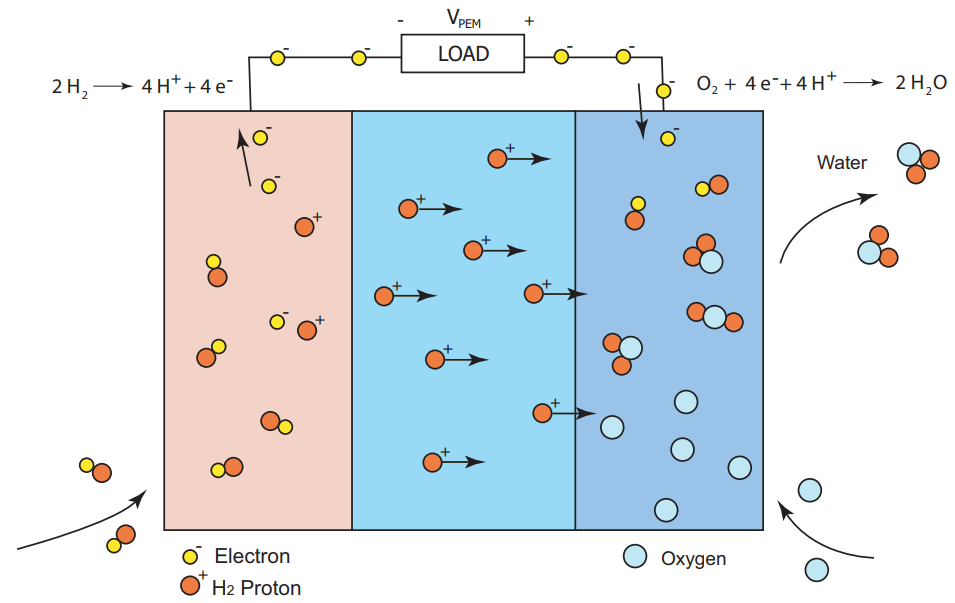
\includegraphics[width=\linewidth]{pemfc_operation.png}
        \caption{Basic electrochemical operation \cite{mohiuddin2018,thomya2011}.}
    \end{subfigure}
    \hfill
    \begin{subfigure}[t]{0.36\linewidth}
        \centering
        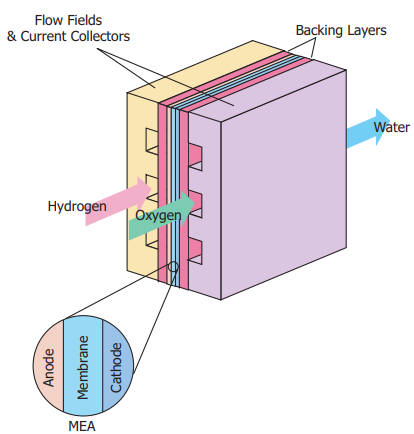
\includegraphics[width=\linewidth]{pemfc_stack_structure.png}
        \caption{Simplified stack structure and MEA \cite{manana2006}.}
    \end{subfigure}
    \caption{Operating principle and physical structure of a PEM fuel cell.}
    \label{fig:pemfc-operation}
\end{figure}

\begin{figure}[H]
    \centering
    \begin{subfigure}[t]{0.48\linewidth}
        \centering
        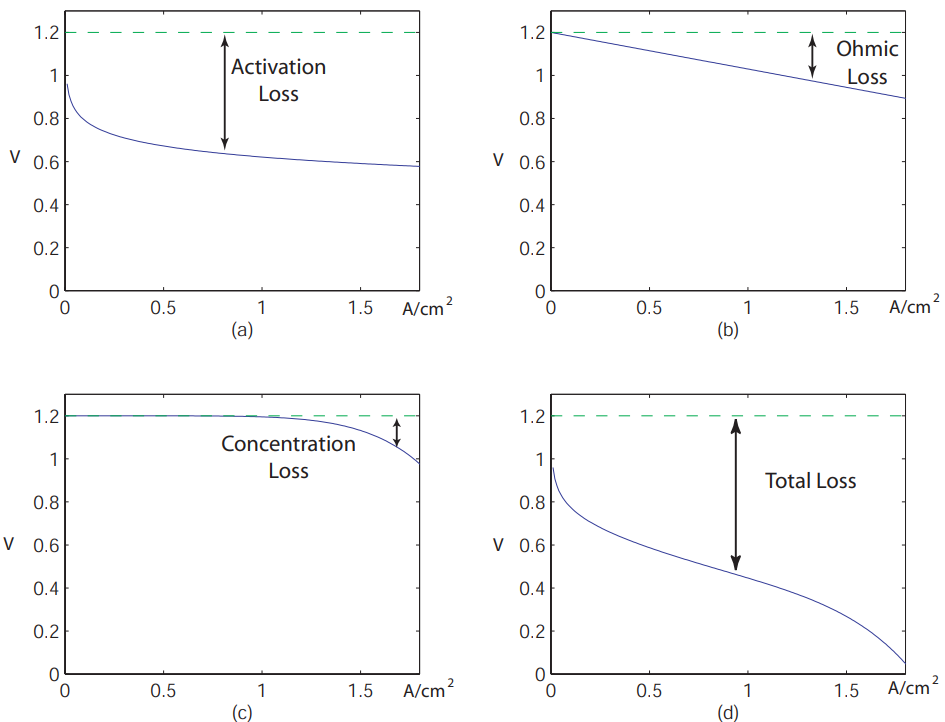
\includegraphics[width=\linewidth]{pemfc_loss_components.png}
        \caption{Activation, ohmic, concentration, and total losses.}
    \end{subfigure}
    \hfill
    \begin{subfigure}[t]{0.48\linewidth}
        \centering
        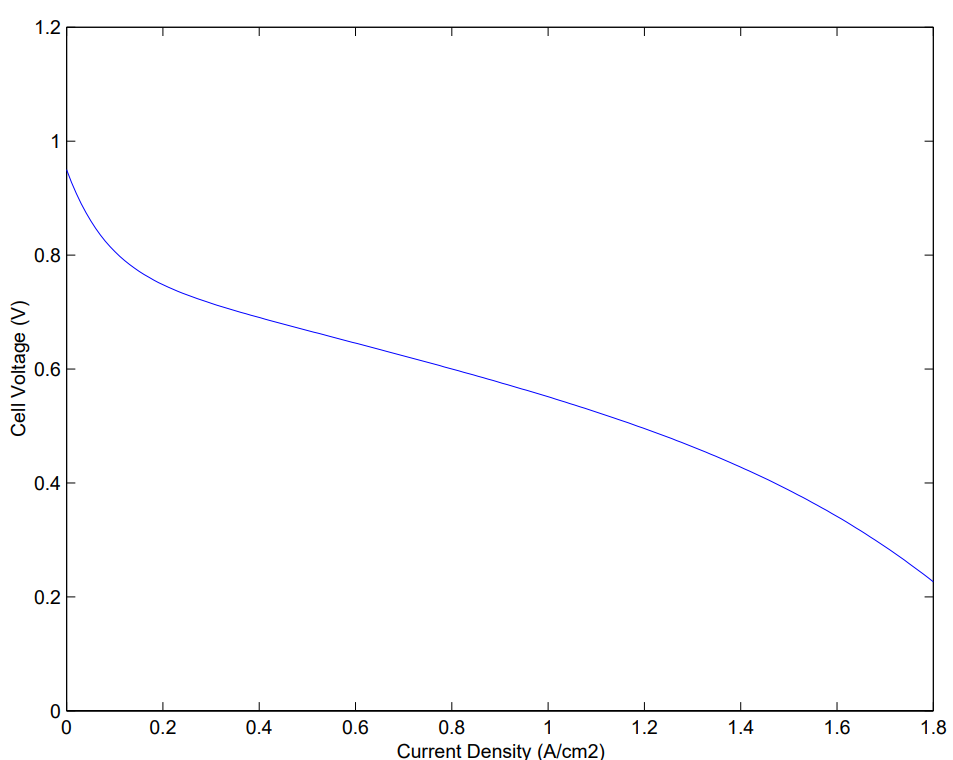
\includegraphics[width=\linewidth]{pemfc_polarization_curve.png}
        \caption{Typical polarization curve.}
    \end{subfigure}
    \caption{Influence of the main voltage losses on PEMFC performance.}
    \label{fig:pemfc-losses}
\end{figure}

\subsection*{B.2 --- Model architecture}

\begin{figure}[H]
\centering
\resizebox{0.95\linewidth}{!}{%
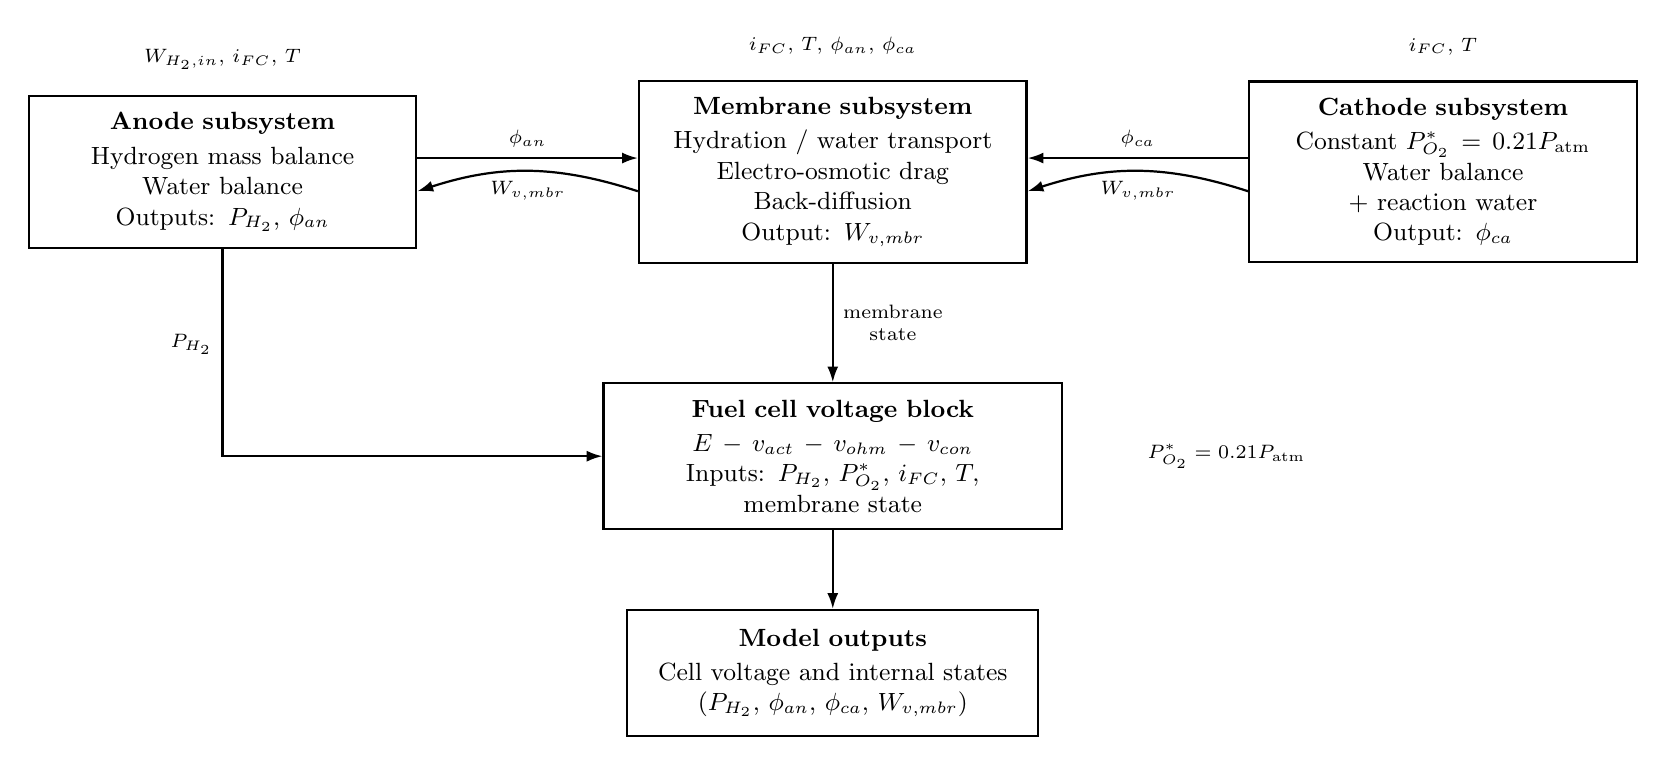
\begin{tikzpicture}[
    >=Latex,
    block/.style={draw, rectangle, thick, fill=white, align=center,
        text width=4.5cm, minimum height=1.9cm, inner sep=6pt, font=\small},
    vblock/.style={draw, rectangle, thick, fill=white, align=center,
        text width=5.4cm, minimum height=1.85cm, inner sep=6pt, font=\small},
    oblock/.style={draw, rectangle, thick, fill=white, align=center,
        text width=4.8cm, minimum height=1.6cm, inner sep=6pt, font=\small},
    lab/.style={font=\scriptsize, align=center},
    line/.style={-{Latex[length=2mm,width=1.4mm]}, line width=0.8pt}
]
\node[block] (anode) {\textbf{Anode subsystem}\\[0.15em]
Hydrogen mass balance\\ Water balance\\ Outputs: $P_{H_2},\,\phi_{an}$};
\node[block, right=2.8cm of anode] (membrane) {\textbf{Membrane subsystem}\\[0.15em]
Hydration / water transport\\ Electro-osmotic drag\\ Back-diffusion\\ Output: $W_{v,mbr}$};
\node[block, right=2.8cm of membrane] (cathode) {\textbf{Cathode subsystem}\\[0.15em]
Constant $P_{O_2}^{\ast}=0.21P_{\mathrm{atm}}$\\ Water balance + reaction water\\ Output: $\phi_{ca}$};
\node[vblock, below=1.50cm of membrane] (voltage) {\textbf{Fuel cell voltage block}\\[0.15em]
$E-v_{act}-v_{ohm}-v_{con}$\\ Inputs: $P_{H_2},\,P_{O_2}^{\ast},\,i_{FC},\,T,$ membrane state};
\node[oblock, below=1.0cm of voltage] (output) {\textbf{Model outputs}\\[0.15em]
Cell voltage and internal states\\ ($P_{H_2},\,\phi_{an},\,\phi_{ca},\,W_{v,mbr}$)};
\node[lab, above=0.2cm of anode] {$W_{H_2,in},\,i_{FC},\,T$};
\node[lab, above=0.2cm of membrane] {$i_{FC},\,T,\,\phi_{an},\,\phi_{ca}$};
\node[lab, above=0.2cm of cathode] {$i_{FC},\,T$};
\draw[line] ([yshift=5pt]anode.east) -- node[above,lab] {$\phi_{an}$} ([yshift=5pt]membrane.west);
\draw[line] ([yshift=-7pt]membrane.west) to[bend right=18]
    node[below,lab] {$W_{v,mbr}$} ([yshift=-7pt]anode.east);
\draw[line] ([yshift=5pt]cathode.west) -- node[above,lab] {$\phi_{ca}$} ([yshift=5pt]membrane.east);
\draw[line] ([yshift=-7pt]cathode.west) to[bend right=18]
    node[below,lab] {$W_{v,mbr}$} ([yshift=-7pt]membrane.east);
\draw[line] (anode.south) |- node[pos=0.23,left,lab] {$P_{H_2}$} (voltage.west);
\draw[line] (membrane.south) -- node[right,lab] {membrane\\state} (voltage.north);
\node[lab, right=0.95cm of voltage] {$P_{O_2}^{\ast}=0.21P_{\mathrm{atm}}$};
\draw[line] (voltage.south) -- (output.north);
\end{tikzpicture}%
}
\caption{Block-level architecture of the reduced PEMFC model.}
\label{fig:architecture}
\end{figure}

\subsection*{B.3 --- Parameter identification, Optimization Experiment}

\begin{figure}[H]
    \centering
    
\includegraphics[width=0.88\linewidth]{cost_evolution_exp19.png}
    \caption{DE optimizer convergence history for all ten cells --- Optimization
             Experiment. Dashed line: final RMSE after L-BFGS-B refinement.}
    \label{fig:cost-evolution}
\end{figure}

\begin{figure}[H]
    \centering
    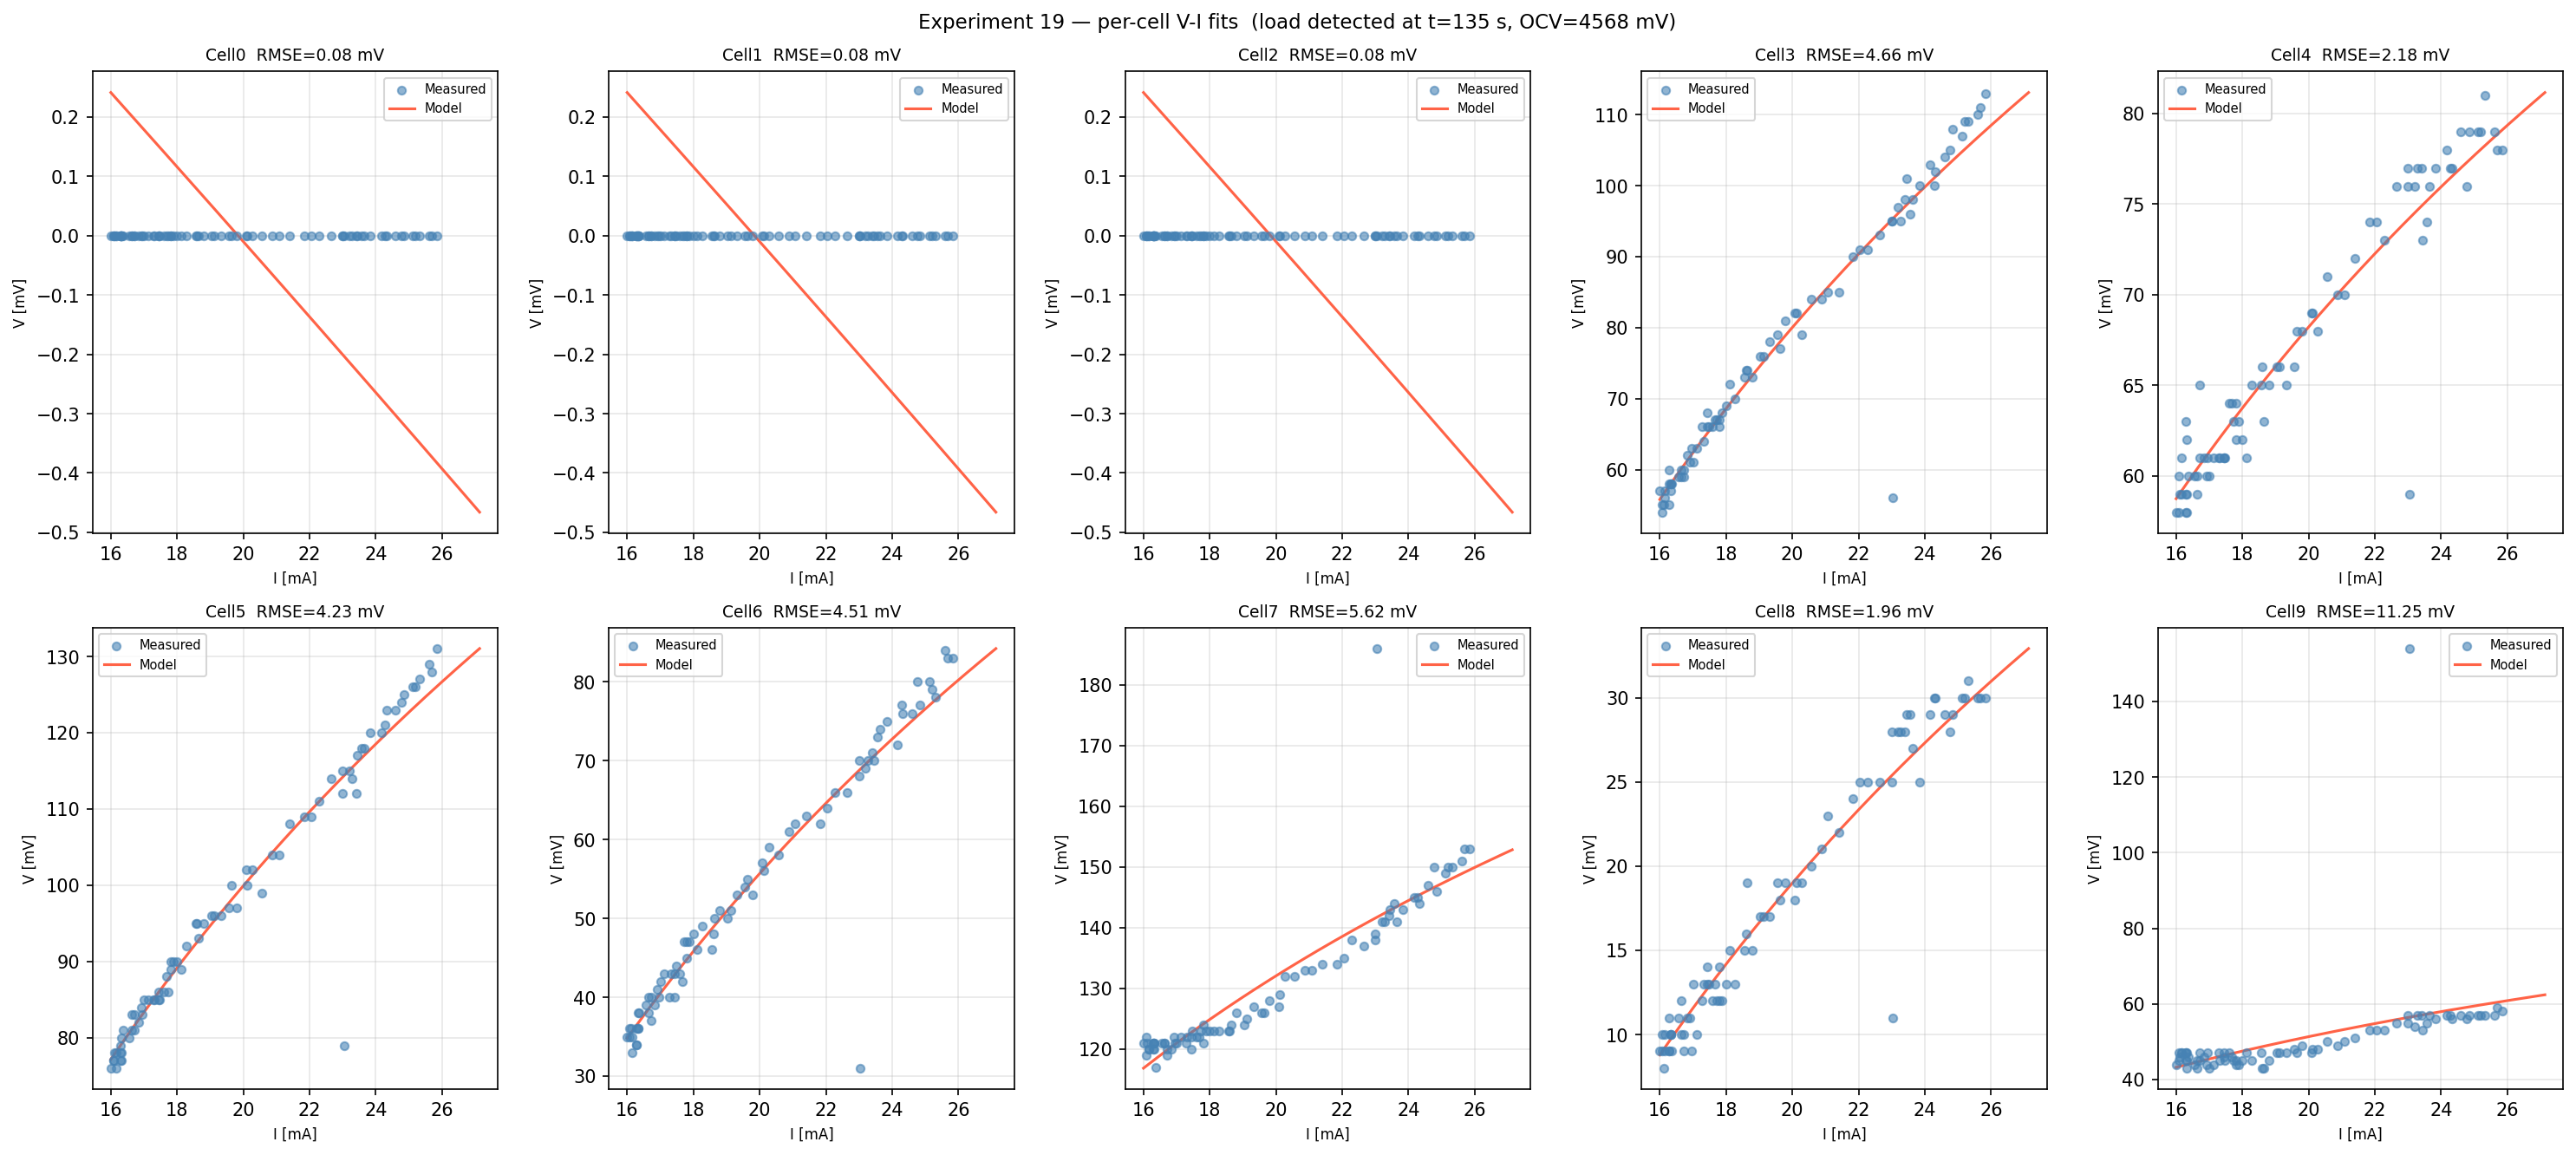
\includegraphics[width=\linewidth]{all_cells_overview_exp19.png}
    \caption{Per-cell $V$--$I$ calibration fits --- Optimization Experiment.}
    \label{fig:vi-opt}
\end{figure}

\begin{figure}[H]
    \centering
    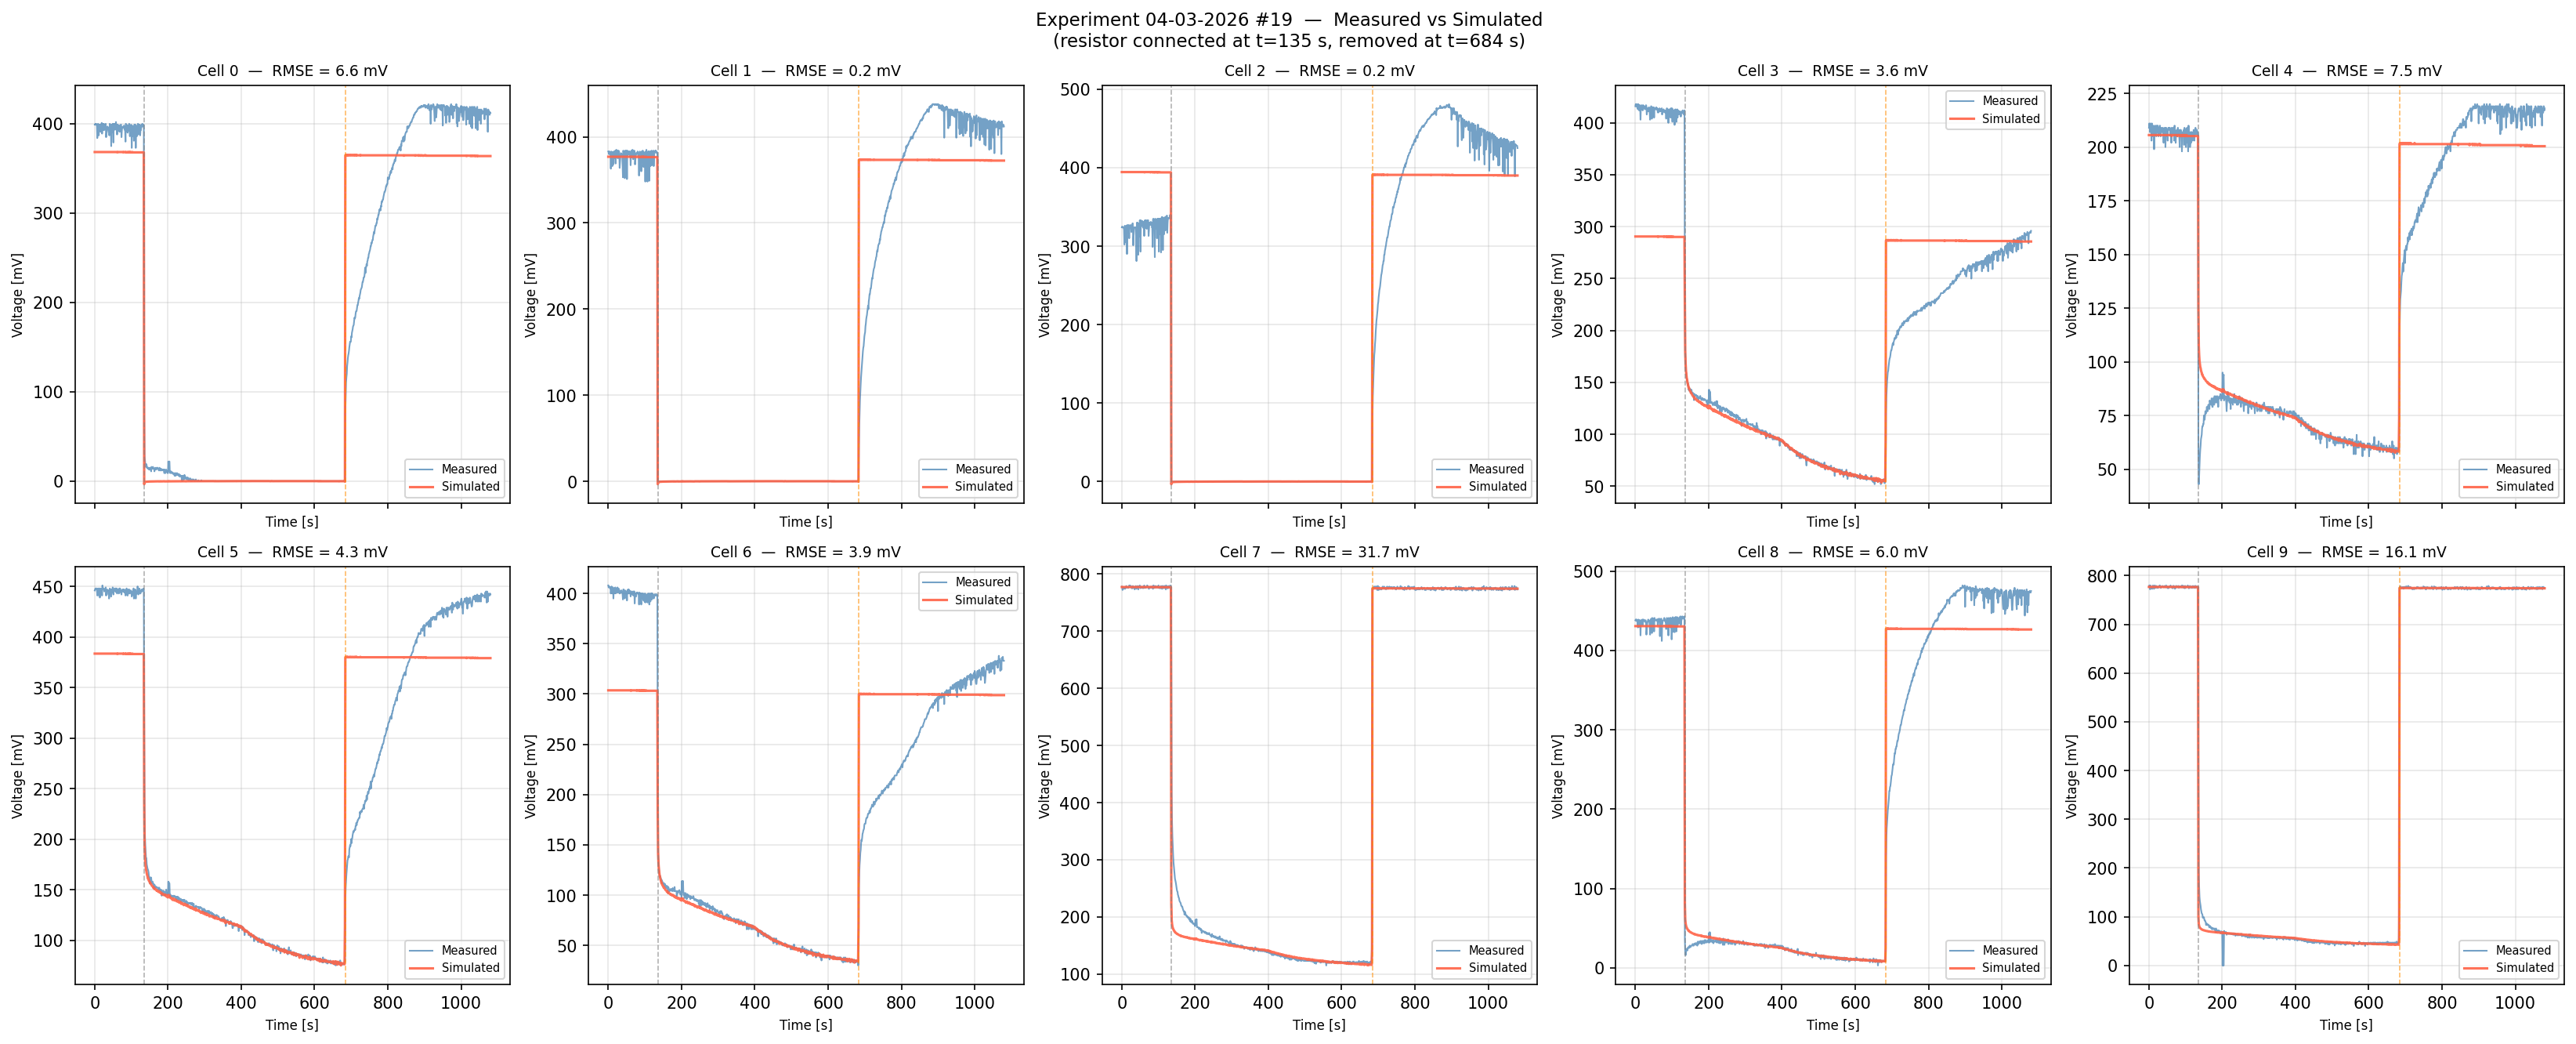
\includegraphics[width=\linewidth]{comparison_exp19_cells.png}
    \caption{Per-cell voltage, measured vs.\ simulated --- Optimization
             Experiment. Cells~0, 1, 2 collapse under load (hardware
             degradation). Mean RMSE (healthy cells) = 8.0\,mV.}
    \label{fig:ts-opt-cells}
\end{figure}

\begin{figure}[H]
    \centering
    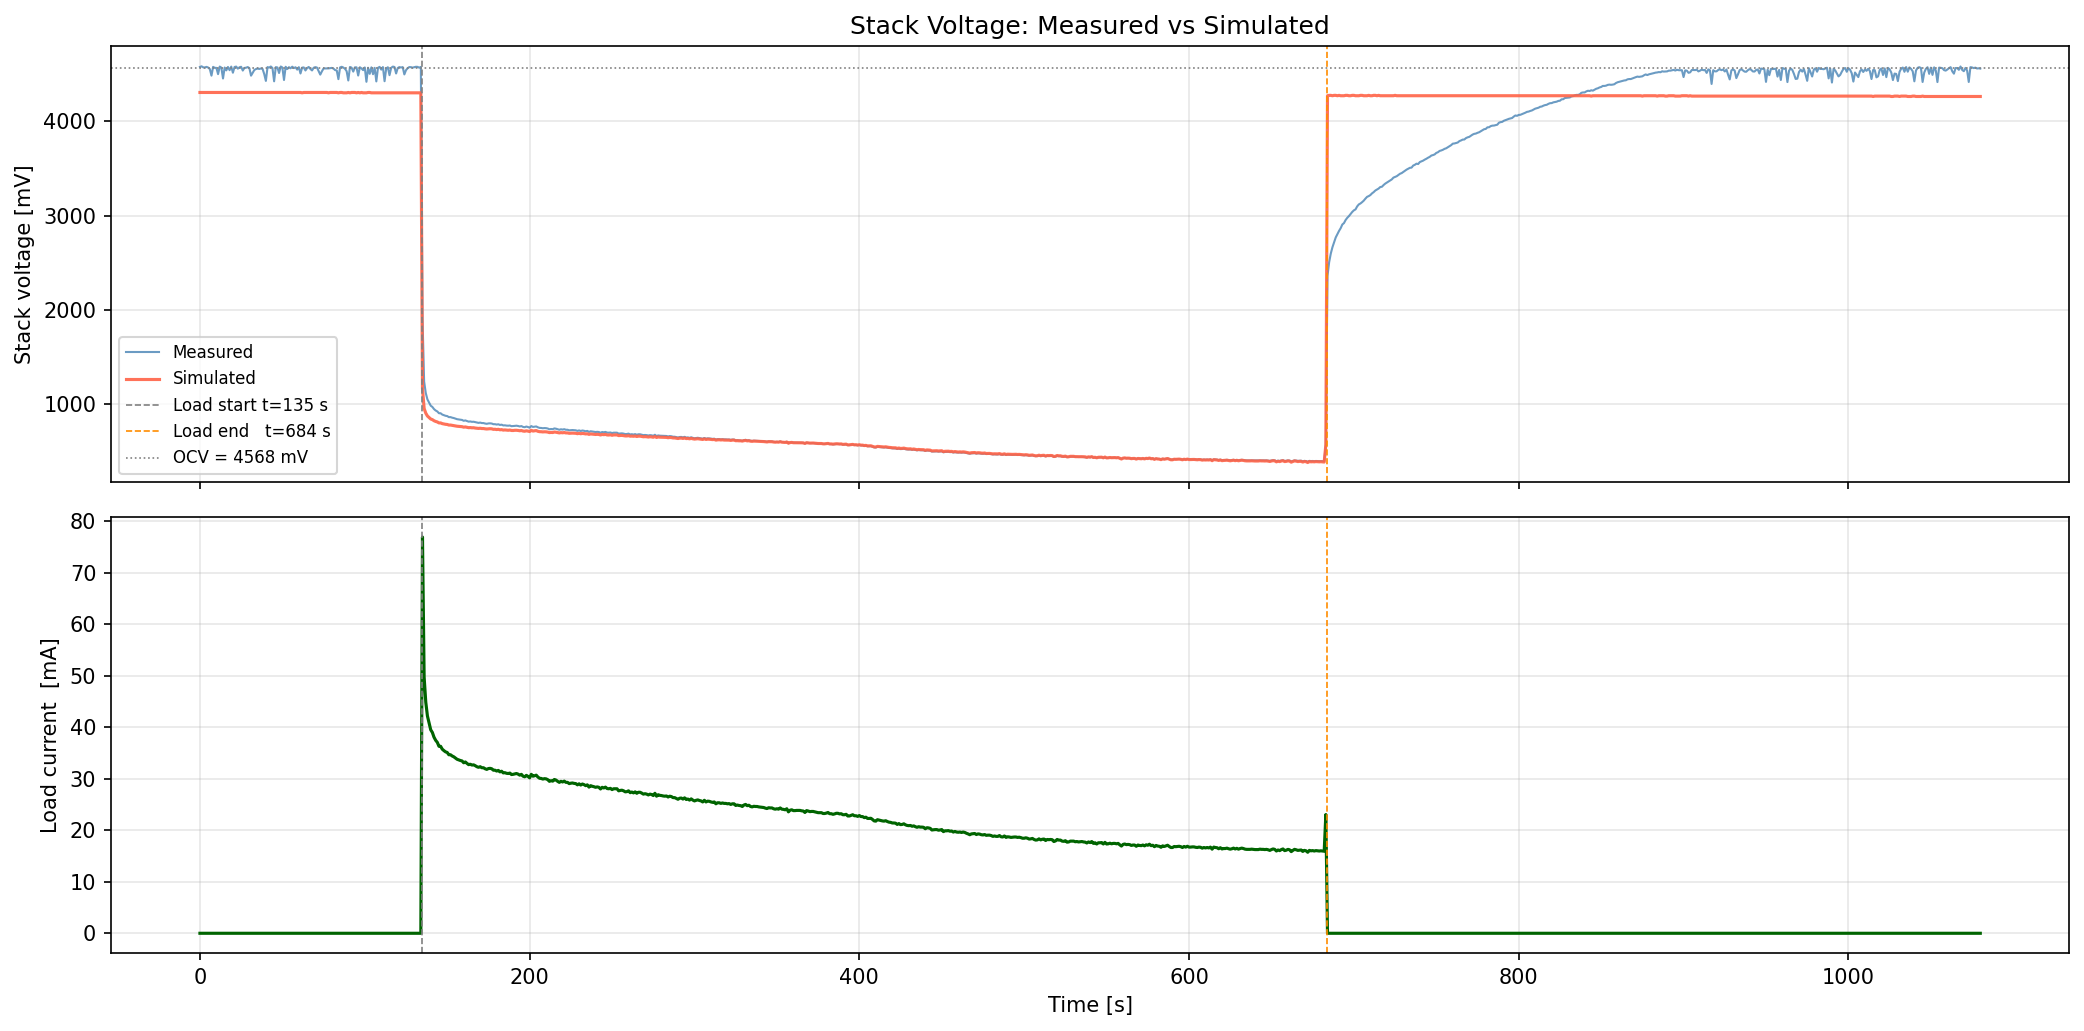
\includegraphics[width=0.85\linewidth]{comparison_exp19_stack.png}
    \caption{Stack voltage, load current and hydrogen pressure --- Optimization
             Experiment. Load applied at $t=135$\,s, removed at $t=684$\,s.}
    \label{fig:ts-opt-stack}
\end{figure}

\begin{figure}[H]
    \centering
    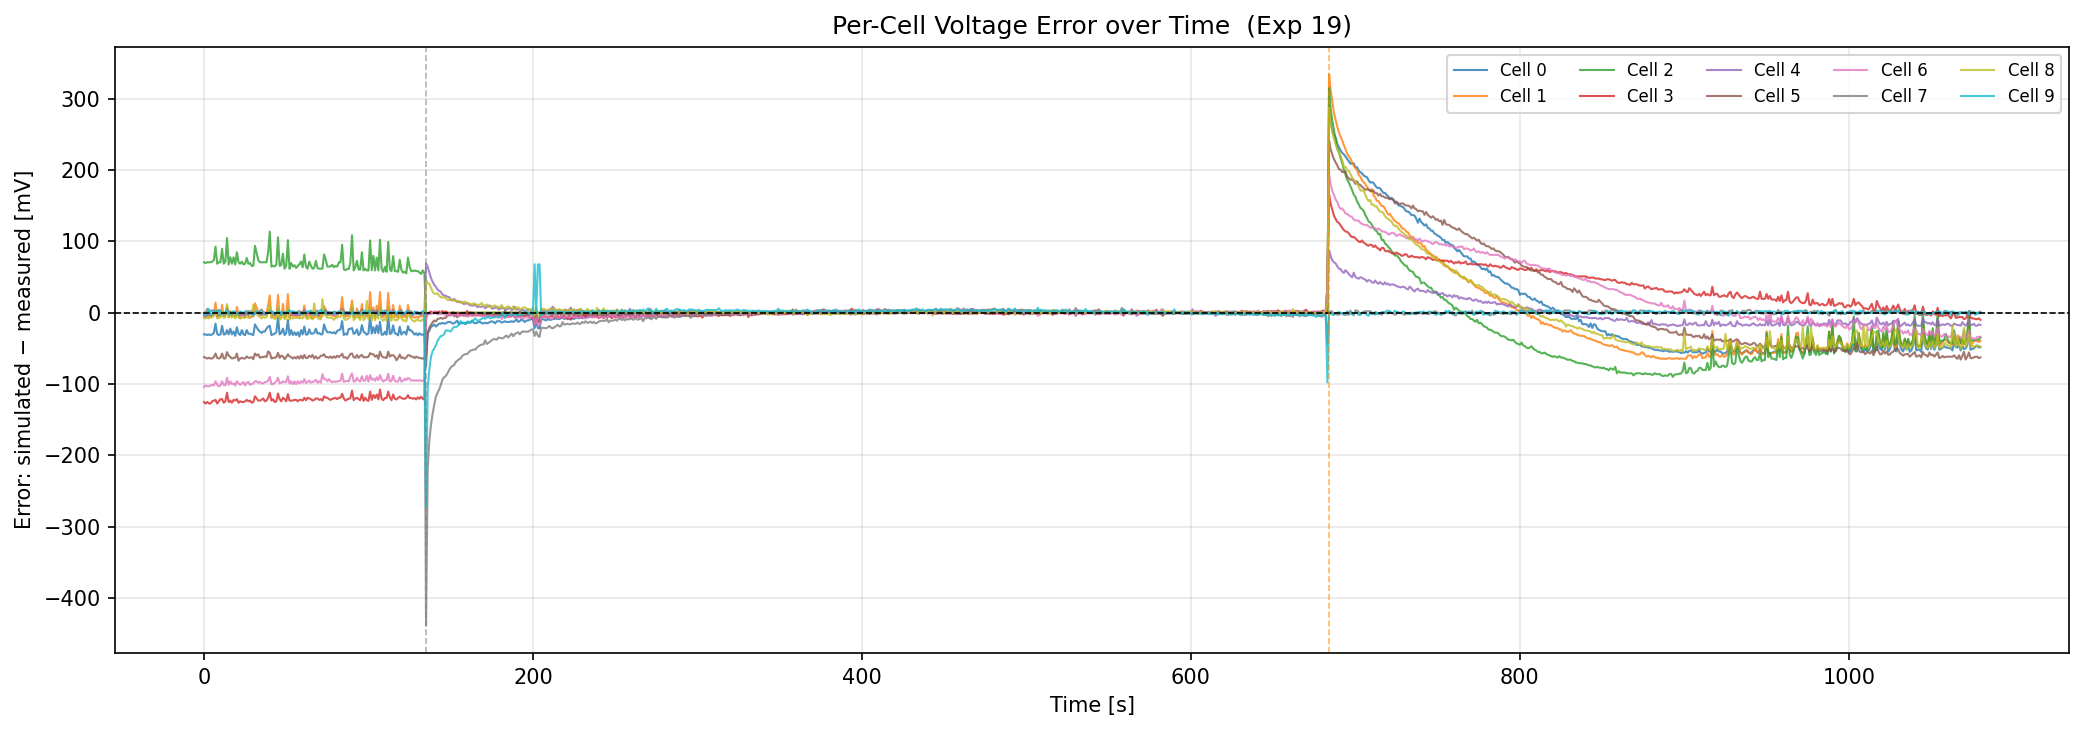
\includegraphics[width=0.85\linewidth]{comparison_exp19_error.png}
    \caption{Per-cell voltage error (simulated $-$ measured) --- Optimization
             Experiment.}
    \label{fig:ts-opt-error}
\end{figure}

\subsection*{B.4 --- TR-current step-response experiments}

\begin{figure}[H]
    \centering
    \begin{subfigure}[t]{0.49\linewidth}
        
\includegraphics[width=\linewidth]{exp_33ohm_plot.png}
        \caption{Experiment~1 ($R=3.3\,\Omega$, 0--250\,s).}
    \end{subfigure}\hfill
    \begin{subfigure}[t]{0.49\linewidth}
        
\includegraphics[width=\linewidth]{exp_68ohm_plot.png}
        \caption{Experiment~4 ($R=6.8\,\Omega$, 0--175\,s).}
    \end{subfigure}
    \caption{TR-current experiments: stack voltage [V], cell voltages [mV],
             current [mA], and power $P=V_{\text{stack}}\cdot I$ [mW].}
    \label{fig:tr-experiments}
\end{figure}

\begin{figure}[H]
    \centering
    
\includegraphics[width=0.72\linewidth]{response_time_plot.png}
    \caption{Current step response after resistor connection: measured data
             (color), exponential fit (dashed), steady-state band, and
             settling-time markers.}
    \label{fig:tr-responses}
\end{figure}

\subsection*{B.5 --- Control architecture}

\begin{figure}[H]
\centering
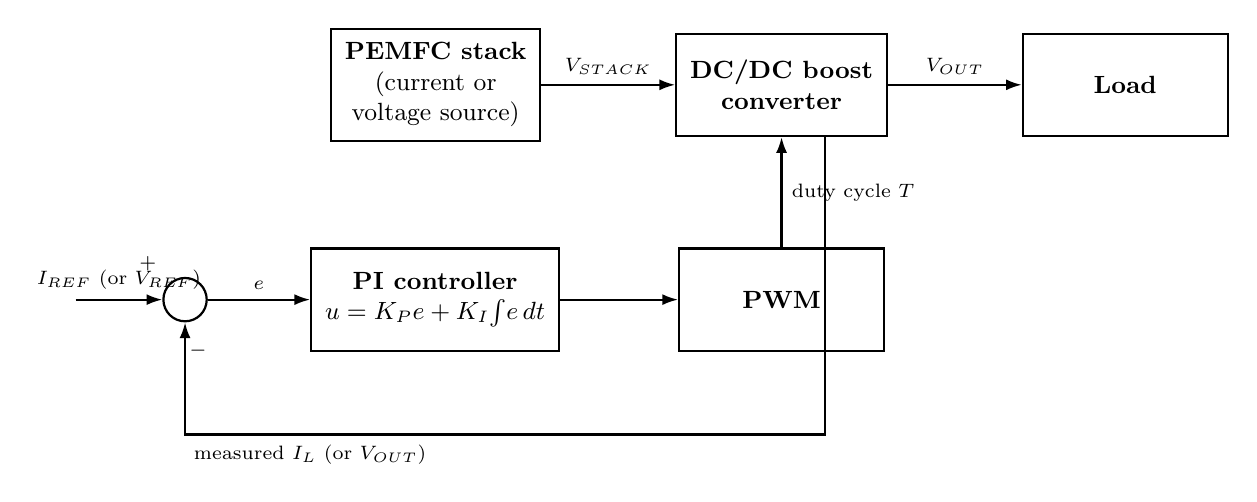
\begin{tikzpicture}[
    >=Latex,
    blk/.style={draw, rectangle, thick, fill=white, align=center,
        minimum height=1.3cm, minimum width=2.6cm, inner sep=5pt, font=\small},
    sum/.style={draw, circle, thick, minimum size=0.55cm, inner sep=0pt},
    lab/.style={font=\scriptsize, align=center},
    line/.style={-{Latex[length=2mm,width=1.4mm]}, line width=0.8pt}
]
\node[blk] (fc) {\textbf{PEMFC stack}\\ (current or\\ voltage source)};
\node[blk, right=1.7cm of fc] (boost) {\textbf{DC/DC boost}\\ \textbf{converter}};
\node[blk, right=1.7cm of boost] (load) {\textbf{Load}};
\node[blk, below=1.4cm of boost] (pwm) {\textbf{PWM}};
\node[blk, left=1.5cm of pwm] (pi) {\textbf{PI controller}\\ $u=K_P e + K_I\!\int\! e\,dt$};
\node[sum, left=1.3cm of pi] (sum) {};
\node[lab, above left=1pt and 1pt of sum.north west] {$+$};
\node[lab, below right=4pt and -2pt of sum.south] {$-$};

\draw[line] (fc) -- node[above,lab] {$V_{STACK}$} (boost);
\draw[line] (boost) -- node[above,lab] {$V_{OUT}$} (load);
\draw[line] (pwm) -- node[right,lab] {duty cycle $T$} (boost);
\draw[line] (pi) -- (pwm);
\draw[line] (sum) -- node[above,lab] {$e$} (pi);
\draw[line] ([xshift=-1.1cm]sum.west) -- node[above,lab] {$I_{REF}$ (or $V_{REF}$)} (sum);
\draw[line] ([xshift=0.55cm]boost.south) |- ([yshift=-1.05cm]pi.south)
    -| node[pos=0.25,below,lab] {measured $I_L$ (or $V_{OUT}$)} (sum);
\end{tikzpicture}
\caption{Control architecture of the PEMFC power system, after
         \cite{derbeli2017}: the stack feeds a DC/DC boost converter whose duty
         cycle is set by a PI controller. Regulating the inductor current $I_L$
         makes the converter output behave as a current source; regulating the
         output voltage $V_{OUT}$ makes it behave as a voltage source.}
\label{fig:boost-architecture}
\end{figure}

% -----------------------------------------------------------------------------
\newpage
\section{Detailed Tables}
\label{app:tables}

\begin{table}[H]
    \centering
    \caption{Tuned parameters and calibration RMSE for all ten cells ---
             Optimization Experiment. Cells~0--2 collapsed under load: the
             optimizer returns identical degenerate parameter sets that
             reproduce a near-zero voltage and are not physically meaningful.}
    \label{tab:params-opt}
    \small
    \begin{tabular}{lrrrrrrr}
        \toprule
        Cell & RMSE [mV] & $\xi_1$ & $\xi_2$ & $\xi_3$ & $\xi_4$ & $B$ & $c$ \\
        \midrule
        Cell~0$^{\dagger}$ & 0.08 & $-7.783$ & $1.67\!\times\!10^{-2}$ & $-6.06\!\times\!10^{-4}$ & $\approx 0$ & $1.08\!\times\!10^{-2}$ & $1.00\!\times\!10^{-2}$ \\
        Cell~1$^{\dagger}$ & 0.08 & $-7.783$ & $1.67\!\times\!10^{-2}$ & $-6.06\!\times\!10^{-4}$ & $\approx 0$ & $1.08\!\times\!10^{-2}$ & $1.00\!\times\!10^{-2}$ \\
        Cell~2$^{\dagger}$ & 0.08 & $-7.783$ & $1.67\!\times\!10^{-2}$ & $-6.06\!\times\!10^{-4}$ & $\approx 0$ & $1.08\!\times\!10^{-2}$ & $1.00\!\times\!10^{-2}$ \\
        Cell~3 &  4.66 & $-1.977$ & $2.83\!\times\!10^{-2}$ & $1.32\!\times\!10^{-3}$  & $-3.17\!\times\!10^{-4}$ & $\approx 0$ & $\approx 0$ \\
        Cell~4 &  2.18 & $ 0.386$ & $1.43\!\times\!10^{-2}$ & $8.11\!\times\!10^{-4}$  & $-1.24\!\times\!10^{-4}$ & $\approx 0$ & $\approx 0$ \\
        Cell~5 &  4.23 & $ 0.682$ & $3.00\!\times\!10^{-2}$ & $1.93\!\times\!10^{-3}$  & $-2.98\!\times\!10^{-4}$ & $\approx 0$ & $\approx 0$ \\
        Cell~6 &  4.51 & $ 1.775$ & $4.62\!\times\!10^{-3}$ & $4.87\!\times\!10^{-4}$  & $-2.73\!\times\!10^{-4}$ & $\approx 0$ & $\approx 0$ \\
        Cell~7 &  5.62 & $ 1.796$ & $2.54\!\times\!10^{-2}$ & $1.82\!\times\!10^{-3}$  & $-1.99\!\times\!10^{-4}$ & $\approx 0$ & $\approx 0$ \\
        Cell~8 &  1.96 & $-4.946$ & $2.81\!\times\!10^{-2}$ & $6.92\!\times\!10^{-4}$  & $-1.34\!\times\!10^{-4}$ & $\approx 0$ & $\approx 0$ \\
        Cell~9 & 11.25 & $-5.400$ & $2.01\!\times\!10^{-2}$ & $9.31\!\times\!10^{-5}$  & $-1.06\!\times\!10^{-4}$ & $3.21\!\times\!10^{-7}$ & $\approx 0$ \\
        \bottomrule
    \end{tabular}

    \medskip
    \footnotesize $^{\dagger}$ Degraded cell (voltage collapse under load); fit not physically meaningful.
\end{table}

\end{document}
